%==============================================================================
% short introduction to get template running on WINDOWS
% further explanation can be found in the pptx
% can be removed after first compilation 
%
% install MikTeX (http://www.miktex.org) - activate auto-install of packages
% install ActivePerl (https://www.perl.org/) - add to HOME
% system reboot
%
% use command-line or IDE in admin-mode to execute the  following commands
% in the specified order (pdflatex used because we want the PDF in the end)
% 
%
% After changes in glossary you need to execute the following command 
% to use the new acronyms
%
% makeglossaries ma_mustermann
%
% After changes in literature you need to execute the following command
% to use the new reference
%
% bibtex ma_mustermann
%
%==============================================================================

% TODO set author and title in header settings

%!TEX root = main.tex
%==============================================================================
% Dokument einrichten und Pakete laden
%==============================================================================

\documentclass[
	pdftex,				% PDFTex verwenden da ausschliesslich ein PDF erzeugt wird.
	a4paper, twoside,	% Verwenden von DIN A4 Papier.
	11pt,				% Grosse Schrift, besser geeignet für A4.
	parskip=half,		% Halbe Zeile Abstand zwischen Absätzen.
	numbers=noenddot,	% Keine Punkte hinter Nummern
	pagesize,           % Schreibt die Papiergroesse in die Datei 
	BCOR=10mm,			% Bindekorrektur
	DIV=13,				% Alternativ 12 oder 14
	headinclude,		% Kopfzeile in den Textbereich
	headsepline,		% Linie nach Kopfzeile.
	openany,            % Keine leere Seite nach/vor neuem Kapitel
	titlepage,
	headings=small,
	bibliography=totocnumbered,	% Bibliographie im TOC nummeriert
]{scrbook}

\usepackage{setspace}\setstretch{1.2} 
%\usepackage{titlesec}

%\titlespacing\section{0pt}{12pt plus 4pt minus 2pt}{0pt plus 2pt minus 2pt}
%\titlespacing\subsection{0pt}{12pt plus 4pt minus 2pt}{0pt plus 2pt minus 2pt}
%\titlespacing\subsubsection{0pt}{12pt plus 4pt minus 2pt}{0pt plus 2pt minus 2pt}

%\usepackage{scrhack}

\usepackage[printonlyused]{acronym}
\usepackage{multicol}

%
% Zeichenkodieruung und Sprache
%

\usepackage[utf8]{inputenc} % Dokument
\usepackage[T1]{fontenc} % Schrift
\usepackage[ngerman, english]{babel}

%
% PDF-Metadaten setzen
%

\usepackage{pdfpages}
\usepackage[
	% Titel des PDF Dokuments
	% TODO set title
	pdftitle={},
	% Autor des PDF Dokuments
	% TODO set author
	pdfauthor={},
	% Thema des PDF Dokuments
	pdfsubject={},
	% Erzeuger des PDF Dokuments
	pdfcreator={},
	% Schlüsselwörter für das PDF
	pdfkeywords={},
	% Dokumenttitel statt Dateiname anzeigen
	pdfdisplaydoctitle=true,																% Sprache des Dokuments
	pdflang=de,
	bookmarksopen=true,
	bookmarksdepth=1,
	colorlinks,
	linkcolor = black,
	citecolor=black,
	urlcolor=black,
]{hyperref}

%
%  Zusätzliche Pakete laden
%

% Anführungszeichen
\usepackage[style=american]{csquotes}

% erweiterte Tabelleneigenschaftn
\usepackage{array, ragged2e}

% Einbinden von Grafiken
\usepackage{graphicx}	

% mathematischer Textsatz
%\usepackage{amsmath}
%\usepackage{amssymb}
%\usepackage{dsfont}

% Textteile drehen
%\usepackage{rotating}	

% Farbpakete
%\usepackage{color}
%\usepackage{xcolor}

% Quellcode sauber formatieren
\usepackage{listings}	

% Font 'Latin Modern Family' verwenden
\usepackage{microtype}
\usepackage{helvet}
\usepackage{mathptmx}

%==============================================================================
% Einstellungen und Definitionen
%==============================================================================

% Farben definieren

\definecolor{light-gray}{gray}{0.95}
%\definecolor{LinkColor}{rgb}{0,0,0.5}
%\definecolor{ListingBackground}{rgb}{0.85,0.85,0.85}
%\definecolor{CommentColor}{rgb}{0, 0.5, 0}
%\definecolor{StringColor}{rgb}{0.63, 0.09, 0.09}

% KOMA-Script Option, Zeilenumbruch bei Bildbeschreibungen.
\setcapindent{1em}

% Stil der Kopf- und Fusszeilen.
\usepackage[headsepline,automark,pagestyleset=KOMA-Script,markcase=ignoreuppercase]{scrlayer-scrpage}
\pagestyle{scrheadings}

% Stil der Überschriften auf normale Schrift.

%\setkomafont{sectioning}{\normalfont\bfseries}		 % Titel mit Normalschrift
\setkomafont{captionlabel}{\normalfont\bfseries}	 % Fette Beschriftungen 
%\setkomafont{pageheadfoot}{\normalfont\itshape}     % Kursive Seitentitel
\setkomafont{descriptionlabel}{\normalfont\bfseries} % Fette Beschreibungstitel

% Codelisting korrekt bezeichnet ausgeben
%\renewcommand\lstlistingname{Source Code}

%==============================================================================
% Listings
%==============================================================================

\lstloadlanguages{% Check Dokumentation for further languages ...
  XML,
  HTML,
  Java,
  Tex
}


\lstset{
  %basicstyle=\scriptsize\ttfamily, % Standardschrift
	basicstyle=\footnotesize\ttfamily,
  %numbers=left, % Ort der Zeilennummern
  %numberstyle=\tiny, % Stil der Zeilennummern
  %stepnumber=2, % Abstand zwischen den Zeilennummern
	%numberblanklines=false,
  numbersep=5pt, % Abstand der Nummern zum Text
  tabsize=2, % Groesse von Tabs
  extendedchars=true, %
  breaklines=true, % Zeilen werden Umgebrochen
  %keywordstyle=\color{red},
  frame=b,
  % keywordstyle=[1]\textbf, % Stil der Keywords
  % keywordstyle=[2]\textbf, %
  % keywordstyle=[3]\textbf, %
  % keywordstyle=[4]\textbf, \sqrt{\sqrt{}} %
  %stringstyle=\color{white}\ttfamily, % Farbe der String
  showspaces=false, % Leerzeichen anzeigen ?
  showtabs=false, % Tabs anzeigen ?
  xleftmargin=17pt,
	xrightmargin=17pt,
  framexleftmargin=17pt,
  framexrightmargin=17pt,
  framexbottommargin=4pt,
  backgroundcolor=\color{white},
  showstringspaces=false % Leerzeichen in Strings anzeigen ?
}

\lstset{literate=%
    {Ö}{{\"O}}1
    {Ä}{{\"A}}1
    {Ü}{{\"U}}1
    {ß}{{\ss}}1
    {ü}{{\"u}}1 
    {ä}{{\"a}}1
    {ö}{{\"o}}1
    {~}{{\textasciitilde}}1
}

\usepackage{caption}
\DeclareCaptionFont{white}{\color{white}}
\DeclareCaptionFormat{listing}{\colorbox[cmyk] {0.43, 0.35, 0.35,0.01}{\parbox{\textwidth-2\fboxsep-2\fboxrule-0pt} {\hspace{15pt}#1#2#3}}}
%\captionsetup[lstlisting]{format=listing,labelfont=bf, textfont=black}

%
% code listing style
%

\lstdefinestyle{kit-cm}{
  backgroundcolor=\color{light-gray},
  belowcaptionskip=1\baselineskip,
  breaklines=true,
  frame=single,
  framexleftmargin=15pt,
  language=C,
  showstringspaces=false,
  basicstyle=\footnotesize\ttfamily, 
  numbers=left,                    
  numbersep=7pt,                
  numberstyle=\tiny\color{black},
  captionpos=b
}

\lstdefinelanguage{Swift}{
  keywords={associatedtype, class, deinit, enum, extension, func, import, init, inout, internal, let, operator, private, protocol, public, static, struct, subscript, typealias, var, break, case, continue, default, defer, do, else, fallthrough, for, guard, if, in, repeat, return, switch, where, while, as, catch, dynamicType, false, is, nil, rethrows, super, self, Self, throw, throws, true, try, associativity, convenience, dynamic, didSet, final, get, infix, indirect, lazy, left, mutating, none, nonmutating, optional, override, postfix, precedence, prefix, Protocol, required, right, set, Type, unowned, weak, willSet},
  ndkeywords={class, export, boolean, throw, implements, import, this},
  sensitive=false,
  comment=[l]{//},
  morecomment=[s]{/*}{*/},
  morestring=[b]',
  morestring=[b]"
}

\lstdefinelanguage{Gherkin}{
	morekeywords = {
		Given,
		When,
		Then,
		And,
		Scenario,
		Feature,
		But,
		Background,
		Scenario Outline,
		Examples
	},
	sensitive=true,
	morecomment=[l]{\#},
	morestring=[b]",
	morestring=[b]'
}

\lstdefinelanguage{json}{
     string=[s]{"}{"},
    stringstyle=\color{blue},
    comment=[l]{:},
    commentstyle=\color{black},
}

\DeclareCaptionFont{black}{\color{black}} 
\DeclareCaptionFormat{listing}
  {\colorbox{white}
     {\parbox{\dimexpr\textwidth-2\fboxsep}{\centering #1#2#3}}}
\captionsetup[lstlisting]{format=listing,labelfont=bf,textfont=black}

\usepackage{hyperref}
\usepackage{paralist}
\usepackage{subcaption}
\usepackage{booktabs}
\usepackage{listings}
\usepackage{caption}




%
% todo notes
%

\usepackage{todonotes}
%\usepackage[disable]{todonotes}	% hide all todo notes
%\presetkeys{todonotes}{inline}{}	% show all defined todos as inline

%
% glossary
%

%\usepackage[acronym,numberedsection]{glossaries}
%\setacronymstyle{long-short}
%\loadglsentries{chapters/glossar}
%\loadglsentries{chapters/glossar.tex}
%\makeglossaries
%\glsdisablehyper
%
% load additional packages
%

\usepackage{calc}
\usepackage{enumitem}
\usepackage{multirow}
\usepackage{mathtools}
\usepackage{enumitem}
\usepackage{amsmath} 
\usepackage{amssymb}
\usepackage{wasysym}
\usepackage{rotating}
\usepackage{pgfplots}
\usepackage{longtable}
\usepackage{algorithm}
\usepackage{algpseudocode}
\usepackage{float}
\usepackage{pdfpages}
\usepackage{threeparttablex}
\usepackage{longtable,lscape}
\usepackage{tablefootnote}
\usetikzlibrary{patterns}
\usepackage{multicol}
\usepackage{bm}
\usepackage{esvect}
%\usepackage{subfigure}
\floatname{algorithm}{Algorithmus}

\makeindex

\usepackage{bera}% optional: just to have a nice mono-spaced font
\usepackage{listings}
\usepackage{xcolor}

\colorlet{punct}{red!60!black}
\definecolor{background}{HTML}{EEEEEE}
\definecolor{delim}{RGB}{20,105,176}
\colorlet{numb}{magenta!60!black}

\usepackage{tabularx}

\usepackage{listingsutf8}
\pgfplotsset{compat=1.16}
\begin{document}

%==============================================================================

%
% add title pages
%

\frontmatter
\setcounter{secnumdepth}{3}
\begin{titlepage}
\thispagestyle{empty}
\enlargethispage{2cm}
%\enlargethispage{\baselineskip}

\sffamily
%\centering
\vspace*{-3.2cm}
\hspace*{-0.6cm}

\includegraphics[height=2.14cm]{figures/kit-logo.png}

\begin{addmargin}{2cm}

\vfill

\begin{tabular}{>{\RaggedRight}p{12cm}}
\begin{center}
{\huge Proseminar}
\end{center}
\\
\begin{center}
{\textbf{\huge K-Means Clustering in Energy Systems}}
\end{center}
\\  
\\
\\
\\
\\
\\
   
\\
{Author: Felix Weik }  \\
{Semester: 5. Bachelor Semester } \\
\\
\\
{Supervisors: Xinyi Wen, TT-Prof. Dr. Benjamin Schäfer}  \\
\end{tabular}
\vfill
\vfill
\vfill



%\singlespacing

\vspace{1em}
\begin{tabular}{ll}
	

	Winter 2023 / 2024 \\
	\\
	\multicolumn{2}{l}{TT-Prof. Dr. Benjamin Schäfer} \\
	\multicolumn{2}{l}{Institut für Automation und angewandte Informatik (IAI)} \\
	\multicolumn{2}{l}{www.iai.kit.edu} \\
	\\
	\multicolumn{2}{l}{\scriptsize{KIT - The Research University in the Helmholtz Association}}\\
\end{tabular}

\end{addmargin}
\newpage
\thispagestyle{empty}
\end{titlepage}	% TODO set author and title
\tableofcontents
%
% add content
%


\mainmatter
%\glsresetall

\chapter{Abstract}
\label{cha:abstract}
Climate change is one of the most pressing issues of our time. 
Researchers in this area are focused on finding solutions to reduce its impact.
One solution can be found in the energy sector, where a large part of the greenhouse gas emissions is produced.
This work focuses on reviewing the application of the k-means clustering algorithm to understand energy load patterns and thus improve the design of energy-saving incentives.
K-means clustering is one of the most popular and widely used clustering algorithms due to its simplicity and efficiency in handling large datasets.
The different papers demonstrate k-means' applications from different perspectives, such as identifying home systems of best practices or reviewing energy efficiency metrics of Chinese industry sectors.
The results show, that k-means works well in finding trends and patterns while handling large datasets efficiently.
This generates knowledge out of the data, which can be used as input for higher-level models or decision-making processes.
Also, k-means weaknesses in this area of usage are analyzed, namely the need for a priori knowledge or the missing ability to spot single outliers in the data.
The algorithm is efficient in its computational complexity, however, multiple executions are needed to evade the risk of local optima.
The research shows that k-means can indeed be used to understand energy load patterns and to improve the design of energy saving incentives.
\chapter{Introdcution}
\label{cha:introduction}

% \begin{itemize}
%     \item Relevance of thesis is explained (Check)
%     \item Give overall context (Check)
%     \item Gap in research is identified (Check)
%     \item Set research questions (Check)
%     \item The Goal of the thesis is formulated clearly (Check)
%     \item How will the problem be addressed (Check)
%     \item brief overview of the paper's structure (Check)
% \end{itemize}

% Explain the relevance of the thesis
Loads of data are created anywhere everywhere all the time.
Yet, due to the lack of actuators collecting and analyzing the data, the data is not fully utilized.
Without proper analysis, the data is just a bunch of numbers.
By analysing the data one can understand the creation process of our most prevalent problems, being able to tackle them at the root.
Without fully understanding the cause of a problem, one can only treat the symptoms.
% Gap in research is identified
A tool to generate knowledge and insights from data is needed.

% Give overall context
This paper introduces the k-means clustering algorithm as a tool to analyse data, and to identify patterns and relations.
K-means is a simple yet efficient, unsupervised machine-learning algorithm that is used to cluster data.
This research is done in a certain context, namely the energy sector.

% Set research questions
After introducing the k-means algorithm and its corresponding data mining techniques, the algorithm is applied to the given context.
The main focuses on two focal research questions:
\textit{How can k-means help to improve the design of energy-saving incentives?} and \textit{Can k-means identify and differentiate natural disaster-impacted load profiles?}.

% Brief overview of the paper's structure + how will the problem be addressed
This work is structured into several chapters, each section reviewing a research question.
These sections focus on the literature review, all in the context of the research question.
First, the k-means algorithm is introduced.
Then, the first research question on the design of energy-saving incentives is reviewed.
This review work will be presented from two perspectives: the perspective of energy efficiency in China's industry and the perspective of behavioral practices in private housing.
Third, the second research question on the identification of natural disaster-impacted load profiles is reviewed.
This review work will deep dive into the energy sector of Lombok, Indonesia.
By reviewing Lombok's climate resilience over several, natural disaster-impacted years, the application of k-means is illustrated.
This work therefore explains how k-means can be used in energy-related research.
\chapter{Background}
\label{cha:background}
% existing methods and concepts are fully introduced
% Mathematics of the methods is correctly covered
% self-developed/chosen solution method is motivated and described fully

% Self-developed / chosen solution method is motivated and described fully
Summarize what the paper aims to do.
How will the following methodological concepts help to achieve the goal of the paper?
Why exactly are these concepts chosen?
What keywords were used to find the papers?
What were the search results?
How will the papers help in answering the research questions?


% Was haben sie in den Papers der Research Questions benutzt?


% Viel aus dem Paper über die Initialisierungsmethoden zitieren, da stehen viele tolle paper drin

% Was möchte ich in diesem Abschnitt vermitteln?
% - Vorstellung von K-Means:
%   - Vorstellung eines generellen Problems
%   - Funktionsweiße mit mathematischen Grundlagen
%   - Die Elbow-Methode
%   - Initialisierungsmethoden
%   - Stärken und Schwächen
%

\section{K-Means Clustering}
\label{sec:k_means_clustering}
% General definition/idea 
Organizing unlabeled data \cite{EZU-CPF} is the general problem of the clustering analysis.
The meaningful grouping of such unlabeled data is regarded as data clustering \cite{ABI-RKC}.
This allows for the identification of patterns and trends in the data, which can be used for further analysis, such as applying more advanced theories and methods.

% Introduce the general problem the algorithm tries to solve
K-means is a partitional clustering algorithm \cite{SIN-UKC}.
It is used to group a set of n data points from z dimensions into k clusters.
This means, that a single partition of the initial dataset is produced with each point being assigned to a distinct cluster \cite{SIN-UKC}.
Clusters are produced heuristically while optimizing a criterion function defined globally on all data objects or locally on the subset of the data objects \cite{ZHU-EPC}.

\subsection{Mathematical Concepts}
As mentioned before, k-means divides a set of n data points from z dimensions into k clusters.
This is done by minimizing the sum of squared distances between a datapoint and its assigned cluster center within the whole cluster \cite{HAR-KMA}.
Doing this globally is an NP-hard problem.
Therefore, the algorithm seeks local optima, such that no point can be assigned to a different cluster and the result converges \cite{SEL-GCT}, \cite{HAR-KMA}.

The initial cluster centers are predefined as explained in \autoref*{subsec:initialisation_methods}.
Next, the means of the initial clusters are calculated.
Then, each data point is assigned to the cluster with the closest mean.
These steps are repeated until the cluster centers do not change anymore or the square sum of errors stays the same for multiple iterations \cite{HAR-KMA}.

\paragraph*{Initialisation Methods:}
\label{subsec:initialisation_methods}
The purpose of the initialization methods is to find the initial cluster centers.
There are multiple methods to do so, for example, \texttt{RANDOM} \cite{PEN-ECI}, the \texttt{Forgy Approach} \cite{AND-CAA}, the \texttt{Macqueen Approach} \cite{MCQ-MCA}, and the \texttt{Kaufman Approach} \cite{KAU-FGD}.

The \texttt{RANDOM} is the most commonly used method due to its simplicity while still being an effective initialization method in terms of convergence speed and robustness \cite{PEN-ECI}.
Therefore it is assumed to be the default initialization method in this thesis.

\paragraph*{Pseudocode}
\begin{enumerate}
    \item The algorithm requires an input matrix of n data points in z dimensions and the initial cluster centers as k points in z dimensions \cite{HAR-KMA}.
          The initial cluster centers are chosen according to the used initialization method as explained in \autoref*{subsec:initialisation_methods}.
    \item The average of each cluster is calculated by using $C_i = (1/M) \sum_{j=1}^{M}x_j$ with $C_i$ being the average of cluster $i$, $M$ the number of points in cluster $i$, and $x_j$ the $j$-th point in cluster $i$ \cite{SYA-IKC}.
    \item Iterate over all data points assigning each point to the nearest cluster center.
          To calculate the distance, the euclidean distance $d = \sqrt{(x_1-x_2)^2+(y_1-y_2)^2}$ is used.
    \item Steps 2 and 3 are repeated until the criterion function converges.
          The criterion function is \begin{equation}\label{eq:sse}E=\sum_{i=1}^{k} \sum_{P \in C_i}|p-m_i|\end{equation} with $E$ being the square error-sum, $p$ the point in space, and $m_i$ the average of cluster $C_i$ \cite{LIU-BDE}.
\end{enumerate}

\subsection{Finding k: The Elbow Method}
The elbow method is a heuristic to find the optimal number $k$ of clusters for a given problem.
It is calculated by plotting the square sum of errors (\autoref*{eq:sse}) against the number of clusters.
The optimal number of clusters is the point where the graph's slope changes the most, which is the so-called elbow \cite{SYA-IKC}.

\subsection{Strengths and Weaknesses}
The actual strengths and weaknesses of the algorithm will be discussed in \autoref*{cha:conclusion}.

\paragraph*{Strengths:}

\paragraph*{Weaknesses:}
Due to the algorithm's greedy nature, the algorithm may converge to a local minimum \cite{JAI-DCB}.
Therefore, multiple runs for a given \texttt{k} value with different initial cluster centers are needed to obtain the optimal cluster result \cite{EZU-CPF}, \cite{BAR-LVG}.

% Was sollen die folgenden beiden sections vermitteln?
%  Wichtig: Vergleichen zwischen verschiedenen Methoden, aber nur bei großen Unterschieden.
%  - Grundlegende Vorstellung der Methoden der Papers
%   - Aus welcher Perspektive gehen die Paper an die jeweilige Fragestellung heran?
%   - Warum verwendet das jeweilige Paper diese Methoden (wie sinnvoll ist das im gegebenen Kontext)? 
%   - Was möchten die jeweiligen Paper erreichen?
%   - In welchem Kontext stehen die Paper (bezogen auf die research questions)?
%   - Wie wenden die Paper k-means an?
%   - Dabei nicht jede Methodik einzeln aufschlüsseln, eher zusammenfassen.
%   - Werden die Daten danach weiter verarbeitet (weiterführende Theorien, ...)?
\section{Methodology of the Research Questions}
As presented in \autoref*{cha:introduction}, two research questions are addressed in this thesis.
Both questions are answered by research papers answering similar questions applying k-means clustering.
The following sections will introduce the methodologies of the papers for each research question, comparing and discussing them.

\subsection{K-Means in the Context of Energy-Saving Incentives}
To answer the first research question, two papers are introduced.
Each paper has a different perspective on the given question, namely the perspective of the industry and the perspective of private households.
\textit{Big data-informed energy efficiency assessment of China industry sectors based on K-means clustering} \cite{LIU-BDE} takes the perspective of the industry.
Using k-means clustering, the paper compares different industry sectors and single companies within these sectors to find high-, medium-, and low-consumption clusters according to different environmental metrics.
\textit{Identifying Home System of Practices for Energy Use with K-Means Clustering Techniques} \cite{MAL-HBP} takes the perspective of private households.
Applying social theory to the results of k-means clustering, the paper identifies different home systems of best practices, explaining how habits, behaviors, and socially shared practices exhibit variation in the way households consume energy.

Both papers differ only slightly in their methodology.
\cite{LIU-BDE} applies k-means to cluster different industry sectors and single companies into high, medium, and low energy efficiency.
Therefore, the value for $k$ is predefined as three.
The used data is the list of all companies trading A shares on the Shanghai (SSE, \url{http://www/sse.com.cn}) and Shenzhen stock exchanges (SZSE, \url{http://www.szse.cn}) since these companies are required to disclose their environmental information every year.
This includes the timespan from 2000 to 2015.
Since the data is noisy, a cleanup of the data is necessary.
After applying k-means, no more theories are applied.
\cite{MAL-HBP} applies k-means to find home systems of best practices (HSOP).
Each cluster found represents a different HSOP.
Therefore, the value for $k$ needs to be adjusted according to each dataset.
Clustering is performed on the data of the Fairwater Living Lab, which delivers data from 39 Australian households from July 1st, 2019 to March 31st, 2021. 
The data is collected by the researchers and includes no noise, therefore no cleanup before applying k-means is necessary.
After applying k-means, the results are further analyzed using social theories and polling the households' residents.

%//TODO: Werden die Daten normalisiert? => evenetuelle Rückschlüsse auf Methodik von Jessen

\subsection{K-Means in the Context of Natural Disaster- and Electrical Fault-Impacted Load Profiles}
%//TODO So umstellen, dass sich relativ wenig wiederholt
One main paper with several sub-papers is introduced to answer the second research question.
\textit{Identification of Natural Disaster Impacted Electricity Load Profiles with k-means Clustering Algorithm} \cite{JES-IND} investigates load profile characteristics and identifies natural disaster impacted load profiles based on k-means clustering for Lombok, Indonesia.
Further aims include the identification of post-natural disaster days capturing the characteristics of natural disaster events.
This helps to understand the impact of natural disasters on the electricity load profile.

The paper's methodology differs in the application of the clusters and the preprocessing.
First, several datasets are collected: The electricity load profiles from 2015 to 2022, and the data on the natural disasters in the same time frame.
The data on natural disasters is provided by the National Disaster Management Agency (BNPB) of Indonesia \cite{BNP-CAD}.
Then, the electricity load profile data is scaled by applying the MinMaxScaler \cite{SKL-MMS}.
For each value $x$ in the dataset is scaled applying \begin{equation}\label{eq:minmaxscaler} 
      x_{transformed} = \frac{x - x_{min}}{x_{max} - x_{min}}
\end{equation} for each of the datapoints \cite{JOJ-ENP}.

After preprocessing, the elbow method and the k-means clustering algorithm are applied as explained in \autoref*{sec:k_means_clustering}.
The clustering is executed on the whole dataset and the year-by-year data.
Each cluster is then labeled as normal or abnormal with abnormal clusters being natural disasters or electrical fault impacted.
This happens by applying the data on natural disasters and checking whether a natural disaster occurred in the given cluster.

% Was ist wichtig in diesem Absatz bzw. was unterscheidet diese Methodik von denen davor?
% - Einführung in die gesammelte Datenmenge => wir haben jetzt zwei Datensätze, auf einem wird geclustert, auf dem anderen werden die Cluster danach analysiert
% - Die Daten werden mit dem MinMaxScaler skaliert
% - Cluster werden mit den Daten zu den Naturkatastrophen gelabeled => Darauf werden dann die einzelnen Naturkatastrophen auf die Climate Resilience des Systems analysisert


% % Data collection
% First, data from 2015 to 2022 is collected and prepared.
% The data collection happens in multiple steps: First, the electricity load data and the natural disaster data are collected.
% The data on natural disasters is provided by the National Disaster Management Agency (BNPB) of Indonesia \cite{BNP-CAD}.
% The paper focuses on earthquakes since they happen the most frequently while having a significant impact on the electricity system.
% Therefore data on the time, the Richter scale severity and the epicenter location of the earthquakes is collected.

% % Data preparation (scaling the data)
% The MinMaxScaler is applied to scale the data to a range of 0 to 1.
% It preserves the shape of the original distribution so the original information is not lost \cite{GOG-WSI}.
% % For each value $x$ in the dataset is scaled applying \begin{equation}\label{eq:minmaxscaler} 
% %       x_{transformed} = \frac{x - x_{min}}{x_{max} - x_{min}}
% % \end{equation} for each of the datapoints \cite{JOJ-ENP}.
% This is done to avoid the influence of the different scales of the data on the clustering result and therefore improves the total clustering performance \cite{GOG-WSI}.
% The optimal number of clusters is found using the elbow method as explained in \autoref*{sec:k_means_clustering}.

% % Seasonal Distribution Analysis
% K-Means is executed on the entire load profile duration and a year-by-year profile duration.
% It is expected to reveal general trends and characteristics as well as precise variations in the load profile.
% After clustering each daily profile will be assigned to a distinct cluster.
% % Separation into normal and abnormal load profiles
% A normal daily electricity load profile is an electricity profile that either resembles the average daily load profile of the specific year in shape and magnitude or is a product of electricity consumer behavior variations.
% An abnormal profile is defined as either experiencing few significant power consumption drops or containing low-magnitude power consumption values that are non-consumer behavior induced.

% % Cluster Labelling
% Clusters are labeled either as disturbance-impacted or normal.
% Disturbance-impacted clusters are either natural disaster-impacted or electrical fault-impacted.
% If a natural disaster does not occur simultaneously with an abnormal load profile, the profile is labeled as electrical fault-impacted.

% % Further analysis of the data regarding climate resilience capability
% After clustering, the data is further analyzed regarding climate resilience capability.
% This means, the data is analyzed in terms of robustness, resourcefulness, and recovery of the electricity system.
% This includes data on the outbreak of the disruption, the impact size, time at the bottom, and recovery duration. and the average restoration rate of the electricity system.


\section{Findings}
\label{cha:findings}
% Grading Criteria
% - Steps taken to arrive at the presented findings are clear 
%       => Das kann auch aus dem Background kommen, es muss nur klar sein wie die Ergebnisse zustande kommen
% - The research question is addressed
% - present findings
% - graphs and table support the main findings 
% - findings are presented without judgment

%//TODO captions der bilder sollen nicht achsen beschreiben, sondern information first, da kann ruhig auch ein haufen stehen

\section{How does the k-means Algorithm help to understand Electricity Load Patterns?}
\label{sec:findings_understand_electricity_load_patterns}
Conducting the literature review provided two different options for choosing the value of $k$ before executing k-means:
By choosing a fixed value the clustering results apply to criteria chosen in advance.
Liu et al \cite{LIU-BDE} choose a fixed value of $k=3$ since the clustering results are divided into low-, medium-, and high-consumption clusters.
By applying k-means with a variable value of $k$ the clustering results adapt to the data and therefore deliver problem-specific results.
This enables Jessen et al. \cite{JES-IND} to spot trends in the data without knowing about certain characteristics in advance.
The clustering results of the whole energy-load profile dataset of Lombok, Indonesia, are shown in \ref{fig:whole_data_clustering_results}.
Each cluster holds approximately the data of a single year, for example, the black cluster contains data from 2015 and the red cluster contains mostly data from 2021.
This shows an overall increase in power consumption over the years.
The algorithm also managed to spot different consumption patterns in the data, with the lime cluster containing mostly the Ramadhan periods from 2018 to 2021.

To further improve the overall understanding of the data, further theories and classifications can be applied after executing k-means.
This classification can take place by taking further datasets into account that underline the found characteristics and patterns.
Jessen et al. \cite{JES-IND} algorithmically label the clustering results into "normal" and "abnormal" clusters, with the abnormal clusters being natural disasters or electrical fault impacted.
This is done by comparing the clustering results with the occurrence time and epicenter of natural disasters and electrical faults.
By reapplying the clustering algorithm to the distinct clusters, the labeling process can be proven.
The clustering results for the earthquake-impacted year 2018 are shown in \ref{fig:clustering_results_2018}.
Again, the algorithm divided the data into distinct clusters, with each cluster representing different consumption patterns.
The red cluster contains post-natural disaster data, which is analyzed in greater detail in \ref{fig:clustering_results_2018_cluster_two}.

These findings show, that k-means proves useful in understanding electricity load pattern datasets without prior knowledge.
By applying k-means, characteristics, patterns, and tendencies are spotted within the data.
The clustering results can be adjusted by choosing different values for $k$.
If a certain theory or defined categories want to be proven a fixed value is useful, to generate hidden knowledge out of large datasets a variable value is more useful.
This lays the groundwork for revealing hidden knowledge in the data, enabling more advanced methods to fully grasp the data's meaning.

\begin{figure}
    \centering
    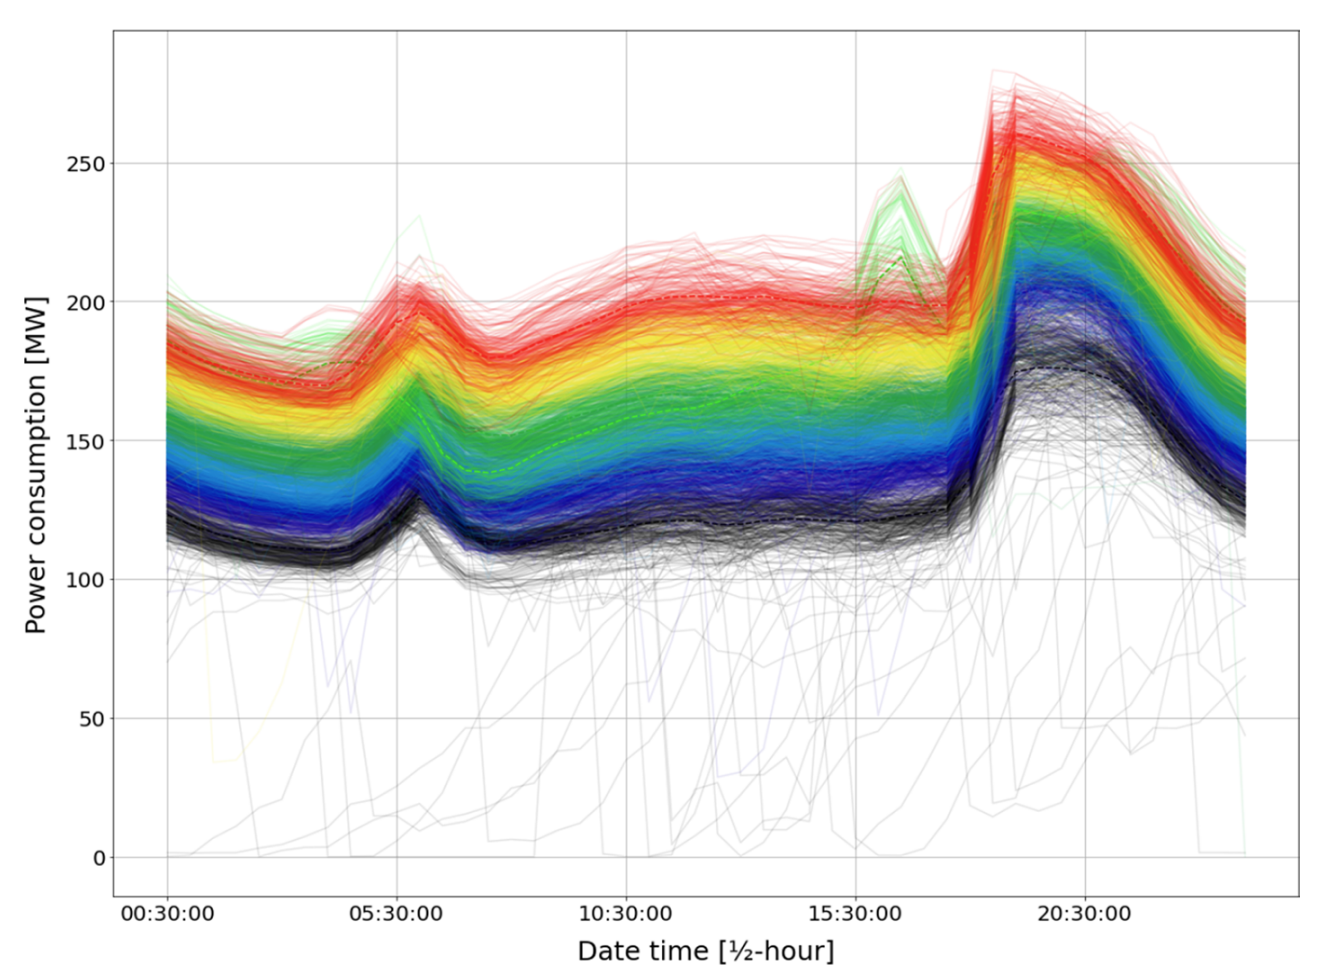
\includegraphics[width=0.6\textwidth]{figures/jessen_ndImpactedClusters/jessen_wholeDataClustering.png}
    \caption{These are the results of executing the k-means algorithm on the whole electricity load profile dataset of Lombok, Indonesia.
    The ideal number of clusters is proven to be $7$.
    Each cluster is represented by a different color.
    Each cluster approximately contains the electricity load profiles of one year.
    It is visible that the power consumption increased over the years since the clusters for the later years are more consuming than the clusters starting from 2015.
    Also, special events like the Ramadhan period are identified, here in the lime cluster.
    }
    \label{fig:whole_data_clustering_results}
\end{figure}

\begin{figure}
    \centering
    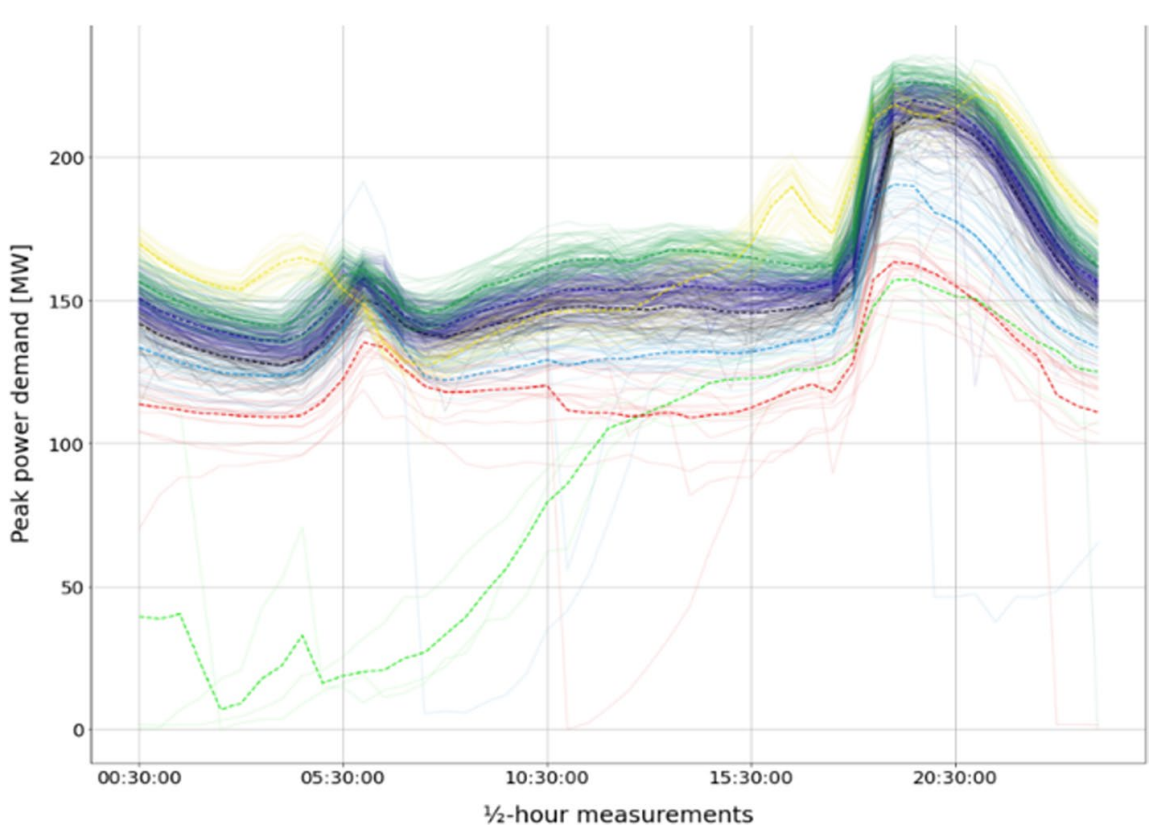
\includegraphics[width=0.6\textwidth]{figures/jessen_ndImpactedClusters/jessen_Clustering2018.png}
    \caption{This is the result of the k-means algorithm applied to the earthquake-impacted year of 2018.
    Again, the ideal number of clusters is proven to be $7$ with each cluster being represented by a different color.
    The clusters are divided into different consumption patterns showing different, non-earthquake-impacted consumption patterns.
    These patterns differ over the year.
    The black cluster contains mid to low-consumption months, mainly from January and February.
    Also, holiday periods like the Ramadhan are identified, here in the gold cluster.
    The algorithm identified the post-earthquake recovery period in the red cluster.
    Also, the dodger blue cluster contains natural disaster-impacted data.
    Both clusters are labeled as "abnormal".
    Therefore, the algorithm successfully identified the earthquake-impacted data from the dataset of an earthquake-impacted year.
    }
    \label{fig:clustering_results_2018}
\end{figure}

\begin{figure}
    \centering
    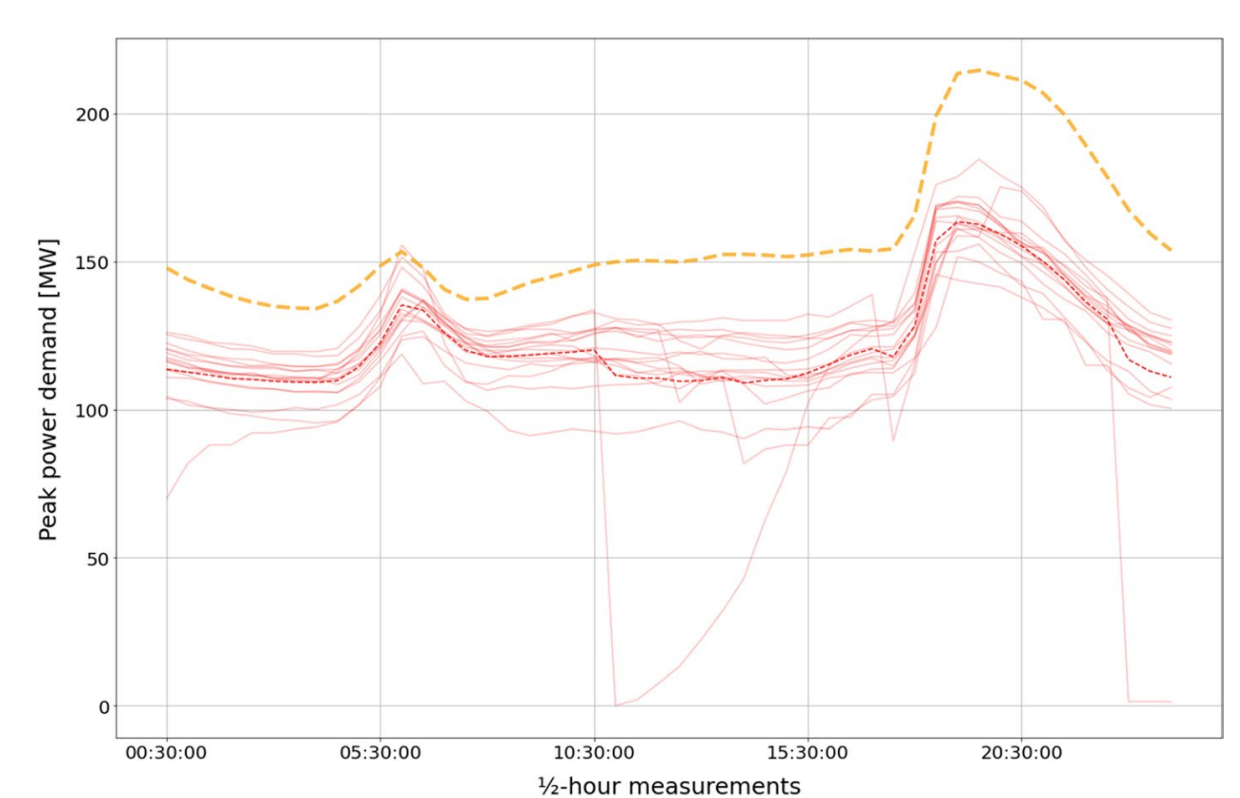
\includegraphics[width=0.6\textwidth]{figures/jessen_ndImpactedClusters/jessen_ClusterTwo2018.png}
    \caption{This figure takes a closer look at the red cluster of the earthquake-impacted year of 2018.
    The Red Solid Lines represent the Clusters' Daily Profiles, the Red dashed Line is the Average for the Red Cluster, and the thick Orange dashed Line is the daily Average for the whole 2018
    It is detectable, that the identified profiles are far from the average daily load profile of the whole year.
    The severe electricity consumption reductions happened as a result of a 7.0 Richter Scale earthquake on the northern part of Lombok on 5 August 2018.
    During the earthquake, the electricity load reduced by 78\% compared to the pre-earthquake consumption.
    The electricity system did not fully recover within a 10-day range.
    }
    \label{fig:clustering_results_2018_cluster_two}
\end{figure}

\section{Improving the Design of Energy-Saving Incentives}
\label{sec:improving_the_design_of_energy_saving_incentives}

% Idee So ausführen, dass diese RQ auf der ersten aufbaut => es muss nicht viel neues erklärt werden

% % 1. Allgemeine Ergebnisse ansprechen
% % 2. Auf ein Beispiel eingehen (in diesem Fall das Clustering und die Tabelle)
% The results are separated into four parts: Clustering for freshwater consumption, the environmental performance measured on the sulfur dioxide emissions, and the energy efficiency performance measured on the coal consumption.
% The k-means algorithm is applied multiple times for each part: once for the whole dataset containing all industry sectors and for each industry sector separately.
% Therefore, distinct companies can be assigned to a cluster and be compared with other companies from the same or different industry sectors.
% One of the clustering algorithm's results is shown in \ref{fig:multi_industries_clustering_result_environemental_performance}.
% A certain threshold most companies remain below can be determined.
% Furthermore, the number of companies in each cluster can be counted and compared.
% The results of the assignments for each industry sector according to the environmental performance are shown in \ref{tab:multi_industries_clustering_results_based_on_the_so2_emission}.
% Some industry sectors show a clear tendency towards a specific cluster, while others are less evenly distributed.
% Therefore, general cluster structures can be identified with industry sectors being ranked by the chosen metric.
% Also, companies within industry sectors can be compared, which helps detect outliers and best practices.

\begin{table}[h]
    \centering
    \begin{tabular}{c|c|c|c|c}
        \textbf{Fields} & \textbf{Sum} & \textbf{Cluster 0} & \textbf{Cluster 1} & \textbf{Cluster 2} \\
        \hline
        Chemical Industry & 144 & 138 & 0 & 6 \\
        Coal Mining and Washing Industry & 60 & 54 & 4 & 2 \\
        Black Metal Smelting & 75 & 53 & 6 & 16 \\
        Textile Industry & 49 & 49 & 0 & 0 \\
        Paper Products Industry & 47 & 42 & 0 & 5 \\
        Electricity, Heat Industry & 384 & 274 & 18 & 92 \\
    \end{tabular}
    \caption{Snippet of the Multi-Industries Clustering Results based on the $SO_2$ Emission \cite{LIU-BDE};
    Each Industry Sector is represented by a Row, the Columns represent the Clusters showing the Number of Companies in each Cluster}
    \label{tab:multi_industries_clustering_results_based_on_the_so2_emission}
\end{table}

\begin{figure}
    \centering
    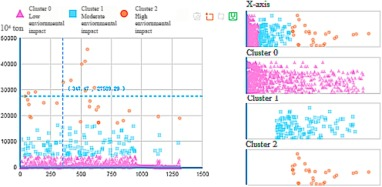
\includegraphics[width=0.6\textwidth]{figures/liu_assessmentOfIndustries/liu_environmentalPerformance.jpg}
    \caption{Multi-Industries Clustering Result based on the $SO_2$ Emission \cite{LIU-BDE};
    Each Point represents a Company its Color represents the Cluster;
    X-Axis: Fuel-Coal Consumption Index, Y-Axis: $SO_2$ Emissions in $10^4$ Tons}
    \label{fig:multi_industries_clustering_result_environemental_performance}
\end{figure}

\begin{figure}
    \centering
    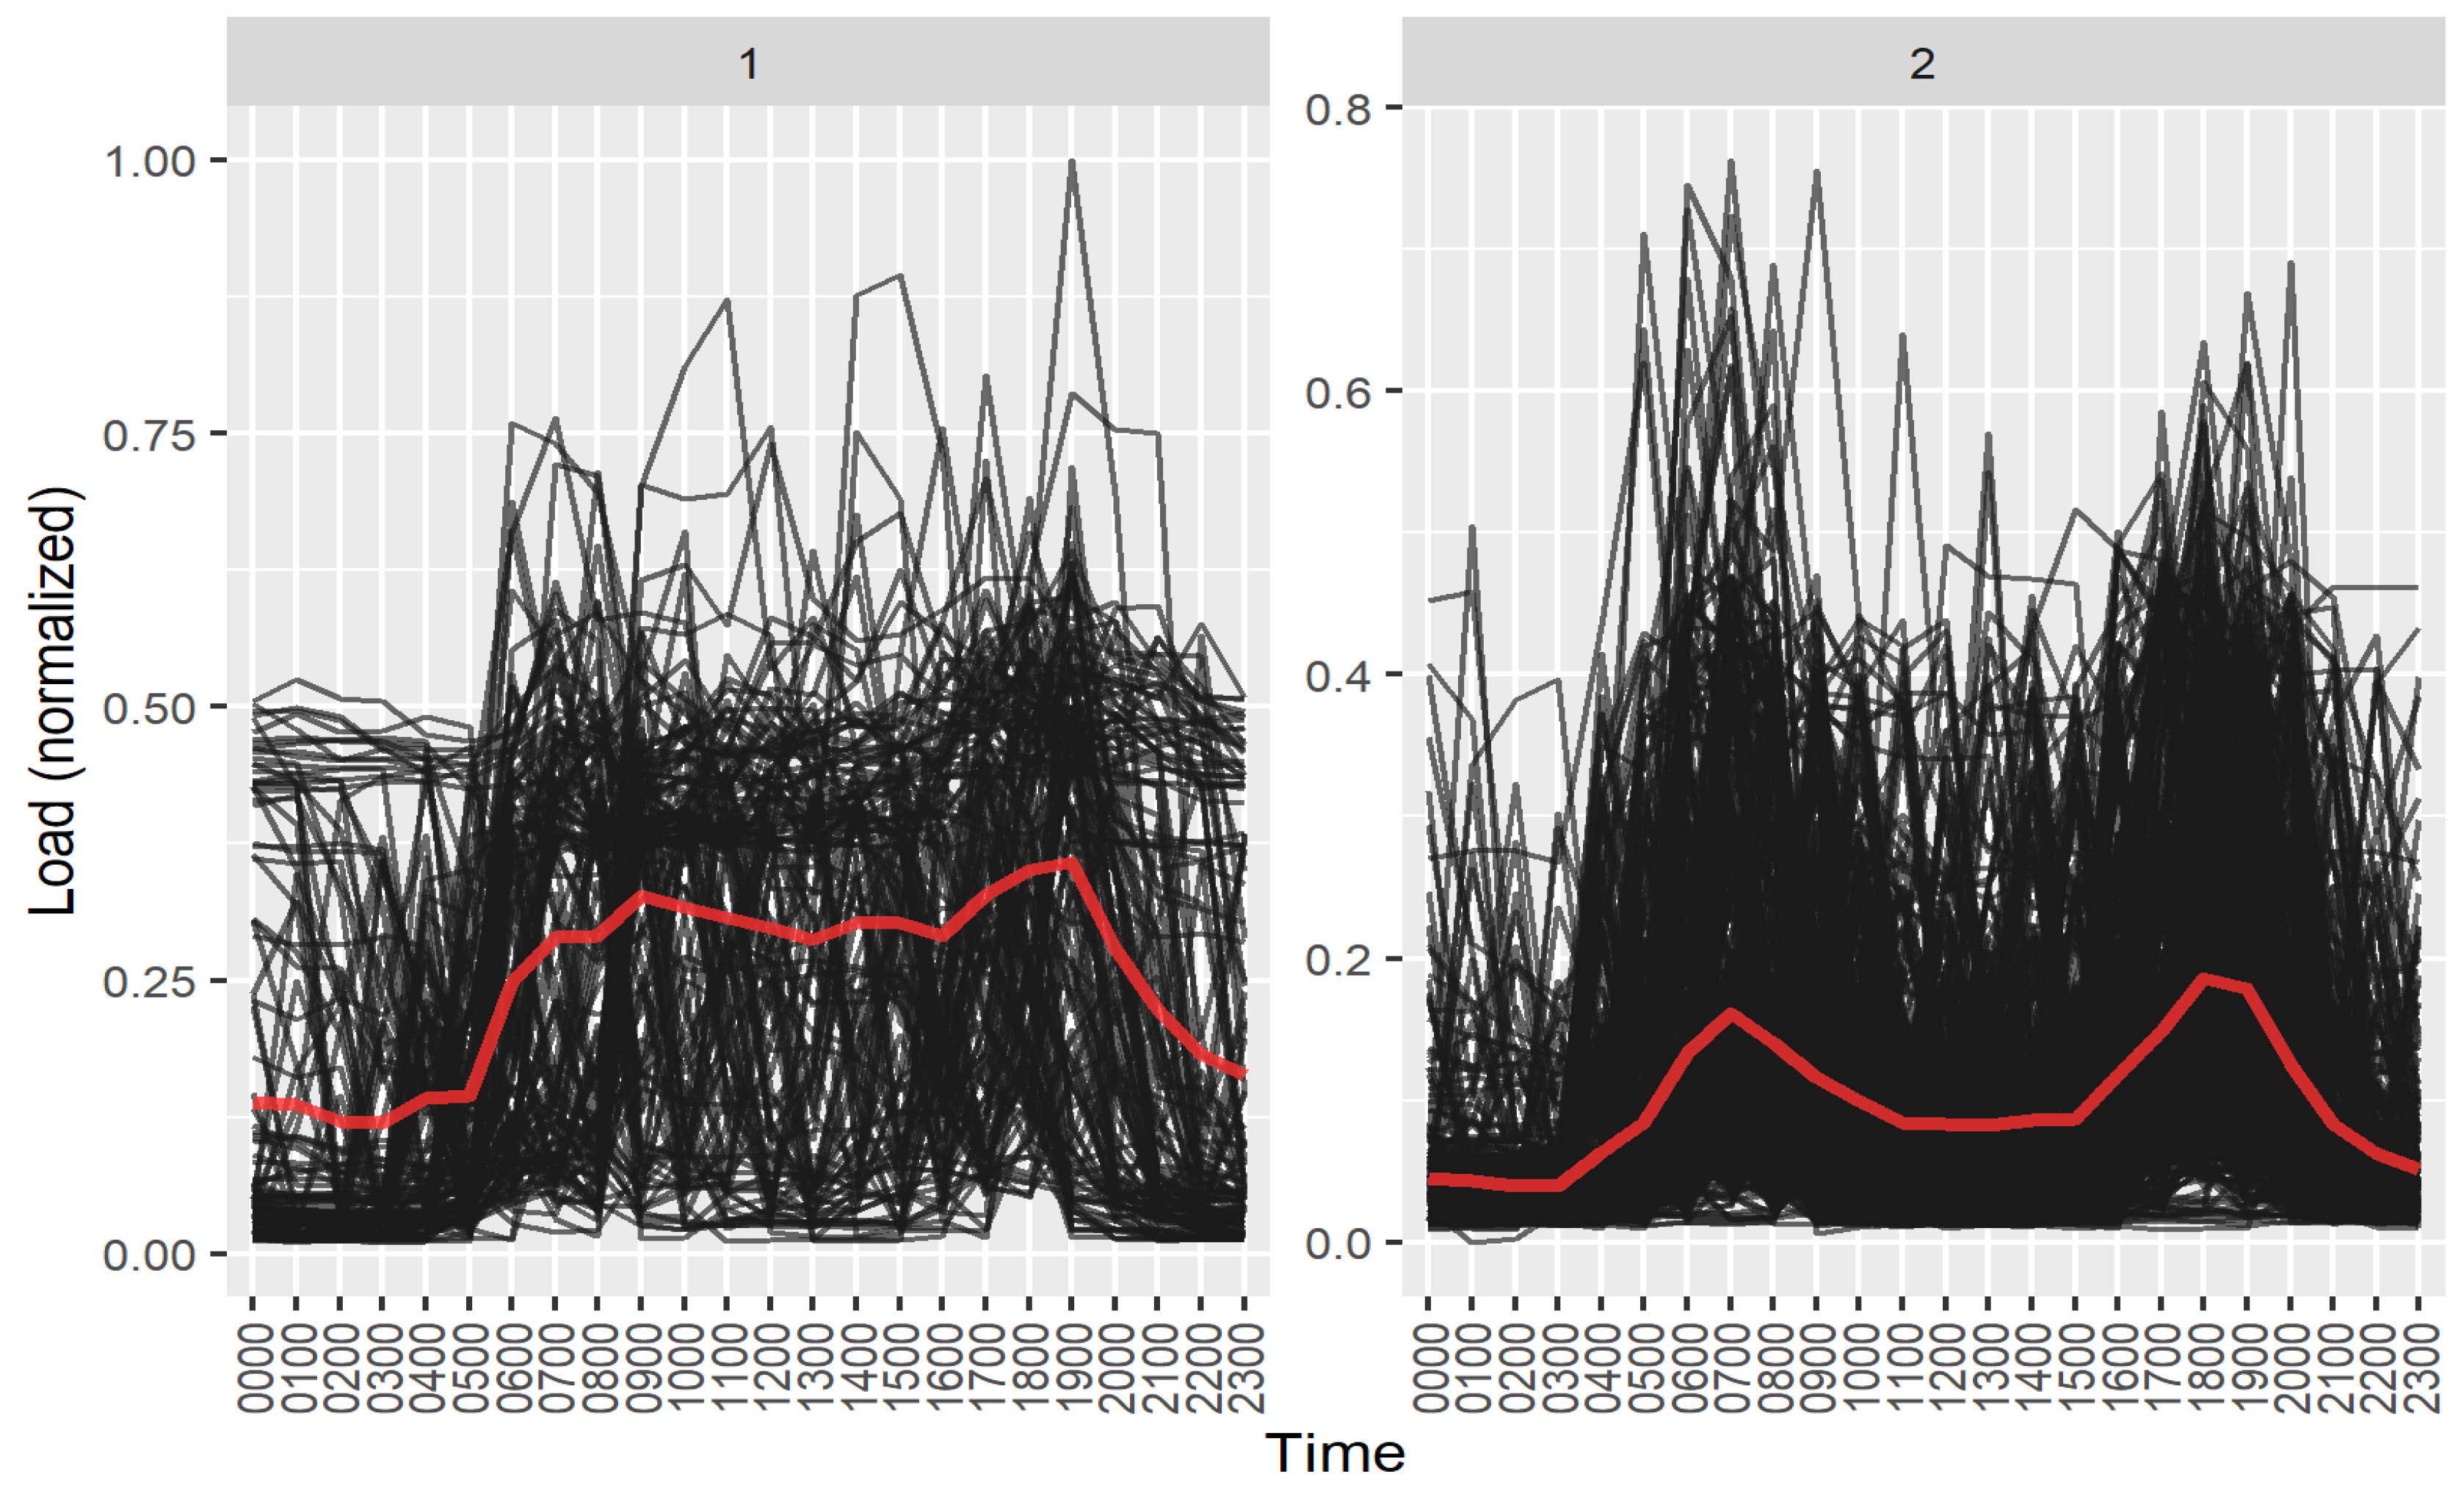
\includegraphics[width=0.6\textwidth]{figures/malatesta_hsop/malatesta_routinisedHousehold.jpg}
    \caption{Single Household Clustering Resulting in a Routinised Household Using all Year Energy Data \cite{MAL-HBP};
    The Red Line represents the Average Consumption in the Cluster, each Black Line represents an assigned Daily Profile;
    X-Axis: Time in 1 Hour Intervals, Y-Axis: Normalized Load Consumption}
    \label{fig:routinized_household}
\end{figure}

\begin{figure}
    \centering
    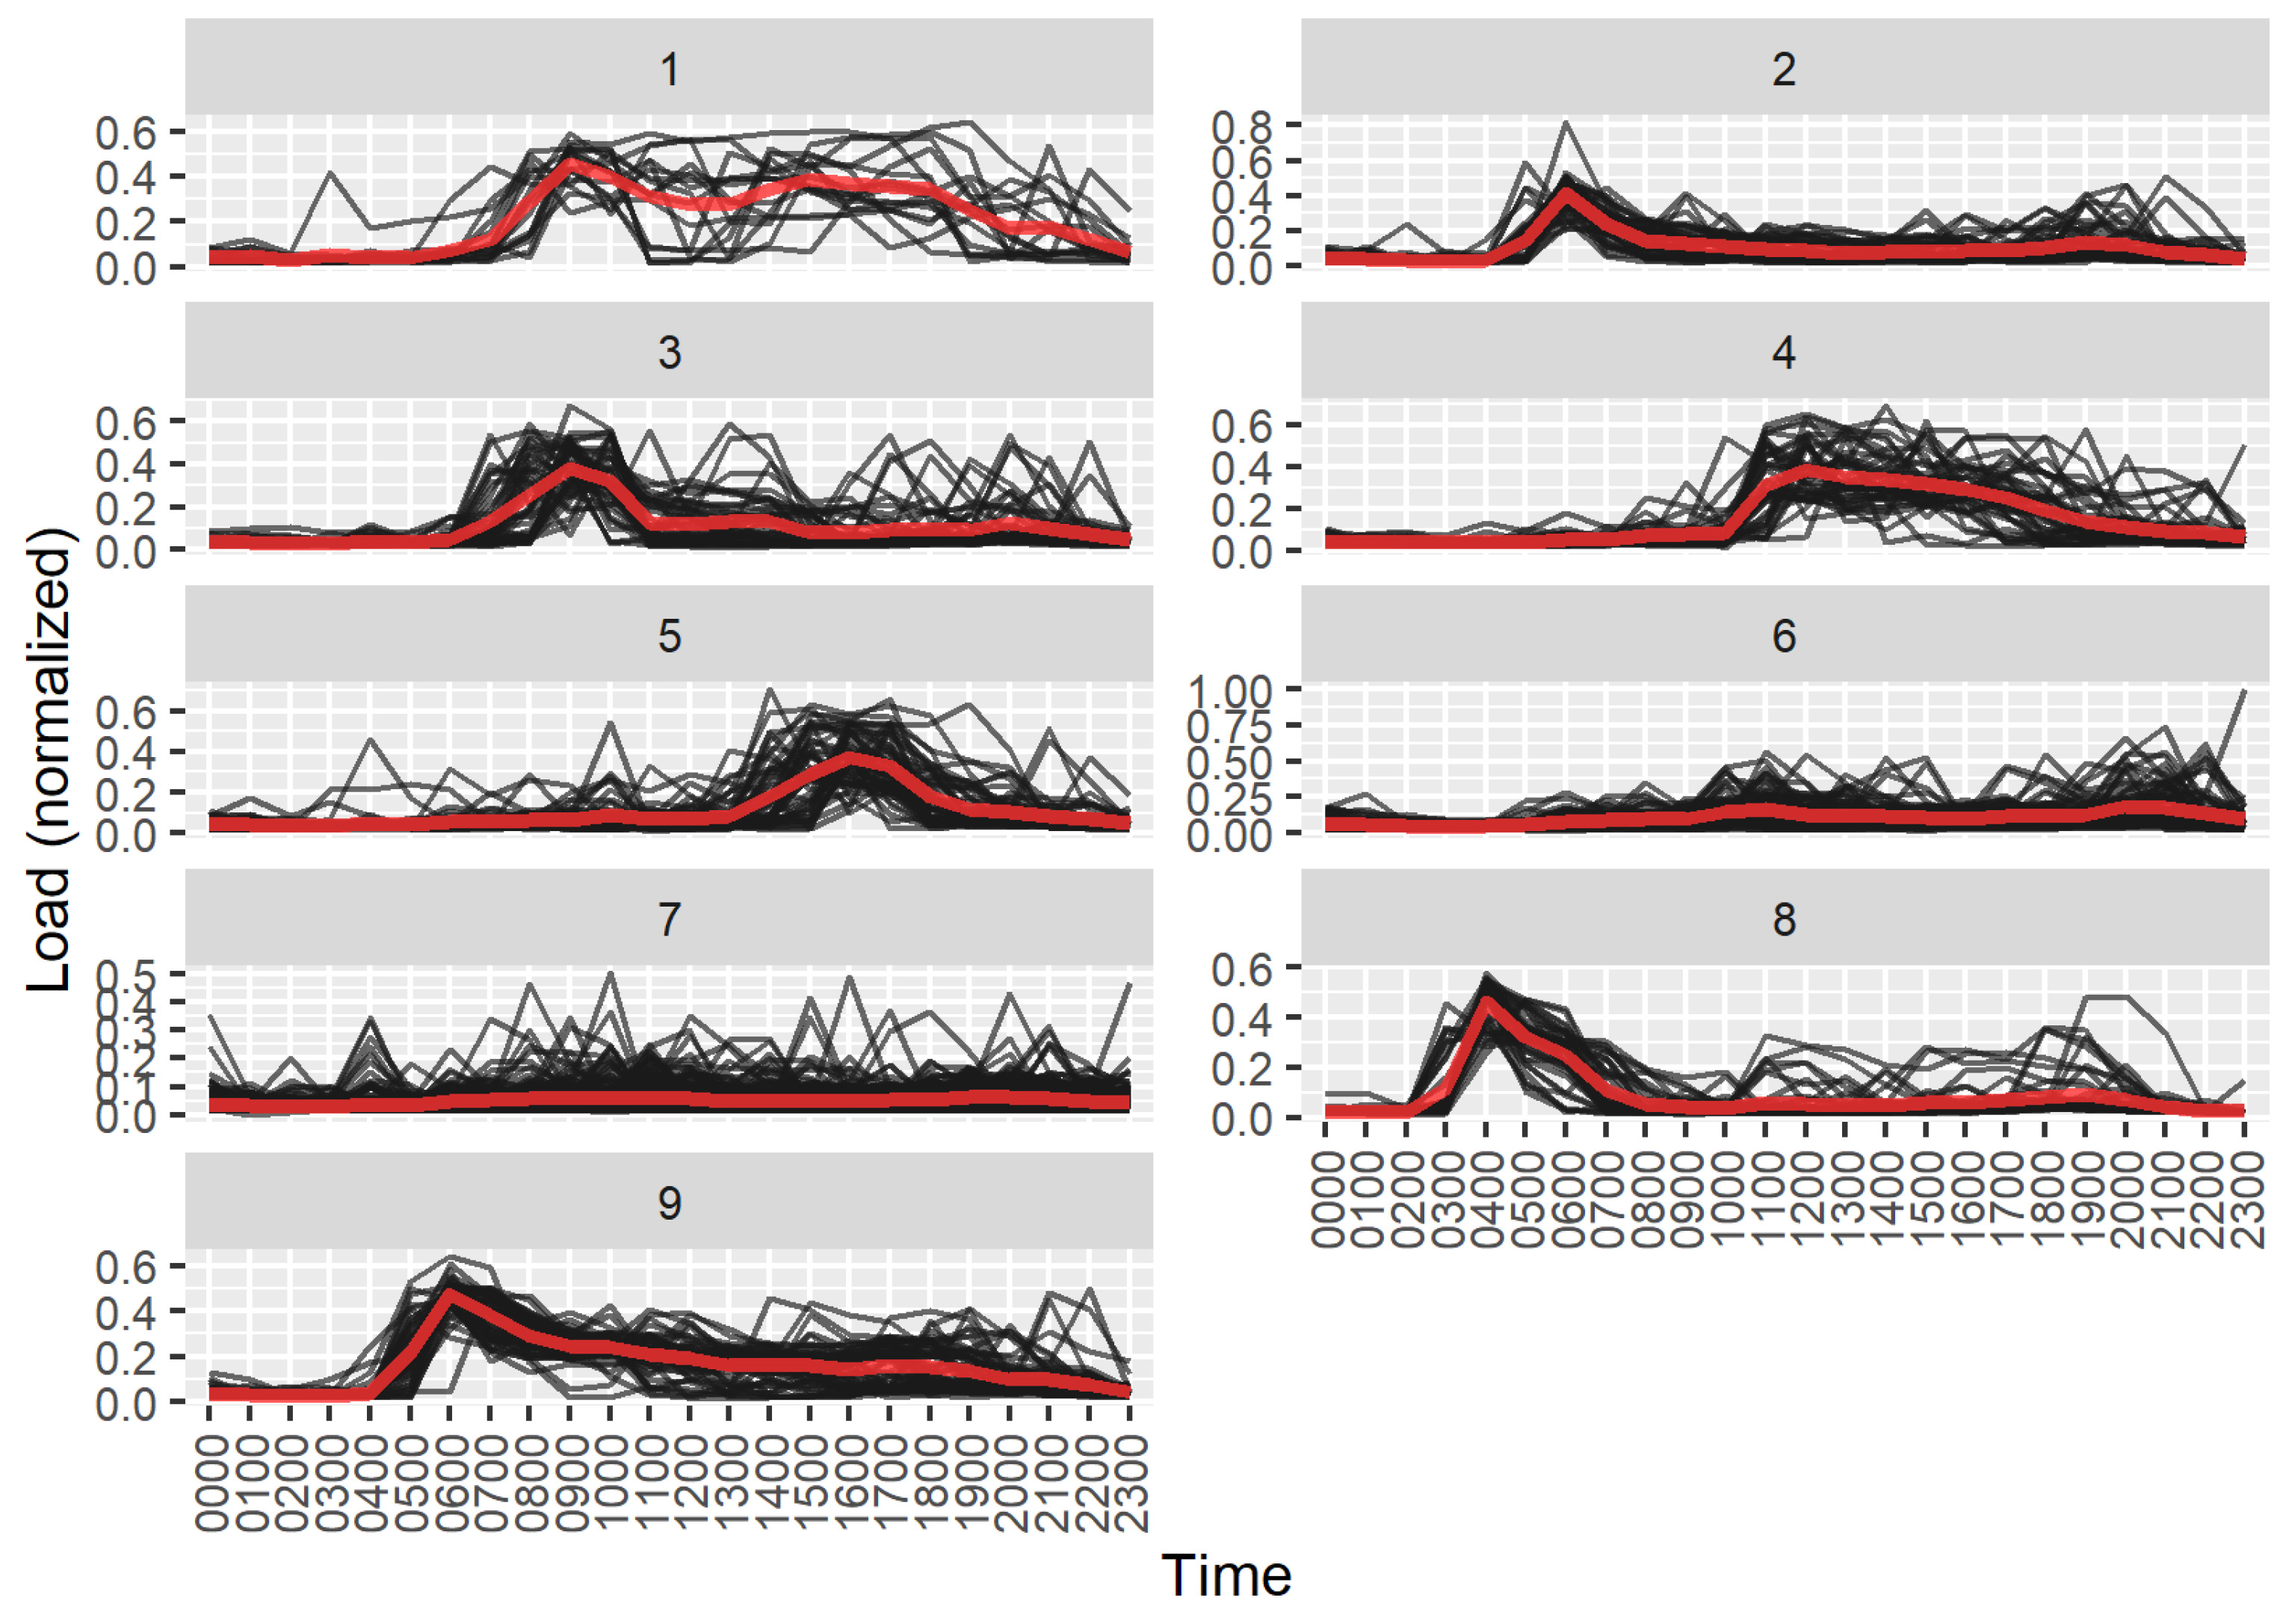
\includegraphics[width=0.6\textwidth]{figures/malatesta_hsop/malatesta_unroutinisedHousehold.jpg}
    \caption{Single Household Clustering Resulting in a Unroutinised Household Using all Year Energy Data \cite{MAL-HBP};
    The Red Line represents the Average Consumption in the Cluster, each Black Line represents an assigned Daily Profile;
    X-Axis: Time in 1 Hour Intervals, Y-Axis: Normalized Load Consumptio}
    \label{fig:non_routinized_household}
\end{figure}

\begin{figure}
    \centering
    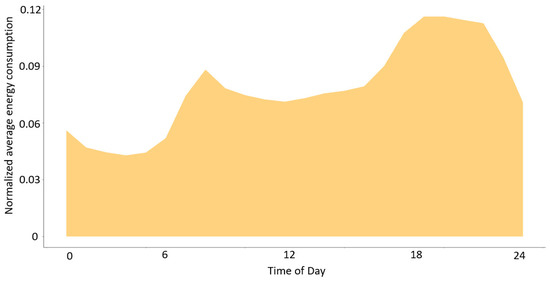
\includegraphics[width=0.6\textwidth]{figures/malatesta_hsop/malatesta_totalDataAveraging.jpg}
    \caption{Result after taking the Average Load Consumption of the Total Dataset \cite{MAL-HBP};
    X-Axis: Time of the Day in Hours, Y-Axis: Normalized Energy Consumption;
    Most Energy Consumption Profiles show a Dual Peak Model with a Dip Midday, the Dominant HSOP}
    \label{fig:total_data_averaging}
\end{figure}

% \paragraph*{MAL-HBP:}
% % Wie soll dieser Paragraph strukturiert sein?
% % 1. Allgemeine Ergebnisse ansprechen
% % 2. Auf ein Beispiel eingehen (in diesem Fall das Clustering und die Tabelle)
% The research is conducted on the total data set and the data split into the disctinct households.
% Also, the data is split into winter and summer data.

% After clustering the whole dataset several assumptions are made.
% First, dominant routines are spotted by averaging the total dataset.
% This leads to a dual peak average as shown in \ref{fig:total_data_averaging}.
% Therefore, practices can be socially shared.
% Also, different consumption practices for the summer and winter seasons are found.

% After applying k-means to each household, routinized households and less routinized households can be identified.
% Routinized households (\ref{fig:routinized_household}) show a smaller number of clusters and therefore less HSOPs than less routinized households (\ref{fig:non_routinized_household}).
% Due to the application of social theories and the survey, two assumptions can be made:
% \begin{itemize}
%     \item Variable lifestyles with different work commitments (e.g. working from home) or family structures (e.g. having children) alter the energy consumption of households \cite{KUR-HBP}.
%     \item If occupants are routinized, their behaviors are repetitive \cite{BRE-EWP}.
% \end{itemize}


% \paragraph*{What do both Summaries have in Common?}
% \begin{itemize}
%     \item Identifying and comparing of:
%     \begin{itemize}
%         % \item Patterns (Malatesta => Habits patterns, clustering of the whole profile; Liu => Some industry sectors are in general more energy consuming than others)
%         % \item Tendencies (Liu => Some industry sectors being represented in cluster 0 and cluster 2)
%         % \item (Best Practices) topic for the conclusion
%         % \item Outliers (Malatesta => Routinised and less routinized households)
%         % \item Shared and individual practices/habits (Malatesta => Whole data clustering)
%         % \item Thresholds (Liu => Limits in consumption/emissions are spotted)
%         \item Characteristics of each cluster (Both => Clusters represent a certain characteristic (Practice/Certain Metric); Malatesta => Some practices can be tracked to a certain practice)
%         \item Dominant characteristics/practices (Malatesta => Some habits reappeared several times in multiple clusterings)
%         % \item Key industries for energy saving incentives (Liu => Some industry sectors are in general more energy consuming than others)
%     \end{itemize}
% \end{itemize}



\paragraph*{Industry:}
% Grundlegende Idee: Ergebnisse in Industrie und Private Housing unterteilen, general findings werden separat für alle Paper gezeigt
% Dabei die jeweiligen Findings am Beispiel zeigen
% Alles was eigentlich aus dem Background klar sein sollte wird dorthin geschoben
% => Nur auf die Ergebnisse aus dem Paper eingehen, dabei nicht werten oder eigene Schlussfolgerungen ziehen
% Die Schritte, wie man zu den Ergebnissen kommt, sollen aus dem Background bereits klar sein
Applying k-means with a fixed value of $k=3$, the datasets are separated into low-, mid-, and highly-efficient industry sectors or companies within these sectors.
Therefore, general patterns are detected and compared.
Spotting these general characteristics' thresholds and characteristic metrics are determined.
A clustering example of the environmental impact measured on $SO_2$ emissions is shown in \ref{fig:multi_industries_clustering_result_environemental_performance}.
General high-consuming, low-efficient industry sectors are spotted, in this case for example the black metal smelting industry as shown in \ref{tab:multi_industries_clustering_results_based_on_the_so2_emission}.
Most clusters are represented in one cluster yet some are scattered over several clusters.
\ref{tab:multi_industries_clustering_results_based_on_the_so2_emission} shows the electric power and heat supply industry as a fitting example.
Mostly this is due to a few companies of the reviewed industry sector being less efficient.
This helps in identifying outliers, which means less efficient sectors and companies.
Therefore, applying k-means to the given dataset helps in finding a starting point in industry sectors and distinct companies for putting energy-saving incentives into action.

\paragraph*{Private Housing:}
Again, patterns are detected using k-means, yet in a different context with different interpretations.
Averaging the whole dataset (\ref{fig:total_data_averaging}) provided insights into dominant practices and habits that are socially shared among the residents of the precinct.
Also, HSOPs are different for the summer and winter seasons due to heating and cooling practices.
These assumptions can be made due to k-means laying the groundwork for applying social theory and the survey results after the clustering process.
The \texttt{dual peak model} with dip midday is the average consumption habit of the monitored precinct.
Analyzing the clustering on the whole dataset gave insights into how habits are shared between different households.
Dominant HSOPs are identified with general characteristics being found.
Clustering single household data gave insights into how flexibility and routine affect different energy consumption practices.
The results varied between two (\ref{fig:routinized_household}) up to nine (\ref{fig:non_routinized_household}) clusters per household.
Due to the application of social theories and surveying the residents, two assumptions are made:
\begin{itemize}
    \item Variable lifestyles with different work commitments (e.g. working from home) or family structures (e.g. having children) alter the energy consumption of households \cite{KUR-HBP}.
    \item If occupants are routinized, their behaviors are repetitive \cite{BRE-EWP}.
\end{itemize}
Therefore, applying k-means to this data reveals the hidden knowledge of HSOPs and identifies starting points for developing best practices in energy consumption.

% discuss limitations of the thesis
% potential next steps

% Was möchte ich in diesem Abschnitt vermitteln?
% - Viele eigene Gedanken einbringen
% - Diskutieren, was eventuell besser gemacht werden kann
%   - Können bessere Ergebnisse mit anderen Methoden erzielt werden?
%   - Ist die Arbeit mit anderen Daten sinnvoll?
% - Hat die gegebene Recherche Einschränkungen?

% A case study with larger shares of renewable energy resources in the energy and capacity mix is recommended to investigate the impacts of natural disasters on the renewable-based electricity system [LIU-BDE]

\section{Discussion}
\label{cha:discussion}

\subsection{Strengths and Limitations of K-Means}
% Grundlegende Idee: Auf Limitations und Findings die Stärken und Schwächen von K-Means ausformulieren
\begin{description}
    \item[Strengths:]
    K-means is simple and easy to use on datasets.
    Multiple libraries and data analysis tools support the usage of k-means, for example, the r software environment.
    Jessen et al. \cite{JES-IND} showed that k-means is an effective tool for spotting general trends in large datasets.
    This also shows that k-means can easily be applied to large datasets like several thousand companies' environmental performance data in Liu et al. \cite{LIU-BDE}.
    With its linear runtime of $O(n * K * I)$ ($n$ being the number of data points, $k$ being the number of clusters, $i$ being the number of iterations), k-means is also fast in runtime.
    Finally, the algorithm converges every time, so a result without endless loops is guaranteed \cite{SEL-GCT}.
    % \begin{itemize}
        %     \item Simple and easy to implement and use since a wide range of libraries and tools are available (for example scikit-learn in Python)
        %     \item Effective in spotting general trends
        %     \item Converges every time
        %     \item Linear runtime of $O(n * K * I)$ with $n$ being the number of data points, $k$ being the number of clusters, $i$ being the number of iterations.
    % \end{itemize}
    \item[Weaknesses:]
    Jessen et al. \cite{JES-IND} showed that k-means sometimes failed to spot single outliers in the dataset.
    Outliers could only be spotted if they followed a general trend or if the dataset had multiple outliers in the same region that could be assigned to a single cluster.
    Since the algorithm converges to local optima, it has to be executed multiple times to ensure the correctness of the results.
    Furthermore, the initialization process is tedious since the number of clusters has to be provided before the algorithm can be executed.
    After finding the optimal number of clusters for the given problem, the initial cluster centers have to be found before being able to execute the algorithm on the given dataset.
    This reduces the speed of the fast-executing algorithm in practice.
    % \begin{itemize}
        %     \item Failed to spot single outliers in the data
        %     \item Tideous initialization process until actual execution takes place
        %     \item Converges to local instead of global optima => needs to be executed multiple times
        %     \item Despite the algorithm being fast in runtime, running it multiple times and initializing/evaluating the results takes time
        % \end{itemize}
    \end{description}
    
% Vergleich zu anderen Algorithmen einbauen
Different clustering algorithms have proven to be more effective in improving the mentioned flaws.
K-harmonic means provides superior clustering results in low dimensions compared to k-means \cite{HAM-ALT}.
MAP-DP (Maximum a Posteriori Dirichlet Process) estimates the number of clusters from the data and therefore does not need the number of clusters to be provided beforehand \cite{RAY-ALT}.
Despite being less effective in runtime, MAP-DP is proven to deliver overall better results than k-means \cite{RAY-ALT}.

\subsection{Limitations of the Thesis}
% Wie kann man die Limitations der Paper und der Findings auf die zu beantwortenden Research Questions und die Motivation anwenden?
% Also welche Aspekte der Research Question weißen Lücken auf oder wurden unzureichend behandelt?
The original motivation was to find and tackle the root causes of climate change in the energy sector by focusing on two factors: analyzing energy load profiles and energy-saving incentives.
The shown papers answered the given research questions to a certain extent.
However, some points were not fully addressed.

First, the papers were biased toward their choice of energy sources.
Lombok's energy load profiles portrayed by Jessen et al. \cite{JES-IND} stem mostly from fossil fuels.
The living lab in Blackwater, Australia, is powered sustainably by solar and using heat pumps \cite{MAL-HBP}.
Also, each paper focused on a single region with its unique cultural and environmental conditions.
Therefore the findings cannot be generalized or applied to other regions.
This concludes that the design of energy incentives cannot be applied universally by this research alone.
More research and test data using different energy sources and portraying different regions and environmental conditions are needed to fully prove the k-mean's effectiveness in designing energy-saving incentives. 

Additionally, it is not communicated to what extent the COVID-19 pandemic affected the research results.
Malatesta et al. \cite{MAL-HBP} found non-routinized patterns due to people working from home, which most likely is a result of the pandemic and people being forced to stay and work from home, adapting to this new situation.
This can distort the results and make them less applicable to normal conditions.
The pandemic also affects the total energy load profiles, which can lead to false clustering results.
Jessen et al. \cite{JES-IND} detected an increasing energy consumption over the years, especially in 2020 and 2021 but did not check whether these results stem from the pandemic or other factors.
Therefore, the results are not fully reliable and need to be re-evaluated under normal conditions.

Finally, the papers did not prove the correctness of the k-means algorithm's results.
Since the algorithm converges towards local optima, the results are not guaranteed to be the best possible solution.
Therefore, multiple executions are necessary to ensure the correctness of the results.
However, none of the papers performed multiple executions.
This can lead to result manipulation since an incorrect result can prove a wrong hypothesis despite the correct one being present.
From the research alone it is not possible to conclude that the k-means algorithm is the optimal choice for designing energy-saving incentives and understanding load patterns in general.


\chapter{Conclusion}
\label{cha:conclusion}

% summarize results, highlight main points
% cover results in the context of original motivation and problem statement
% "so what" message is formulated (key take homes, how does it help the reader in the future)
% discuss how the thesis addresses original questions

% Hauptaussage: K-Means ist toll um Trends zu spotten oder erste Eigenschaften aus einer Datenmenge herauszulesen, 
% allerdings kann man diesen Algorithmus nicht blind auf jedes Problem anwenden

% \subsection{Strengths and Weaknesses}
% The actual strengths and weaknesses of the algorithm will be discussed in \autoref{cha:conclusion}.

% \paragraph*{Strengths:}

% \paragraph*{Weaknesses:}
% Due to the algorithm's greedy nature, the algorithm may converge to a local minimum \cite{JAI-DCB}.
% Therefore, multiple runs for a given \texttt{k} value with different initial cluster centers are needed to obtain the optimal cluster result \cite{EZU-CPF}, \cite{BAR-LVG}.




\bibliographystyle{cmnat}
\bibliography{ressources}

%==============================================================================

\end{document}